\chapter{Solución con sensores IMU\label{sec:IMU}}
%------------------------------
%------___SOLUCIÓN_IMU___------
%------------------------------

\label{sec:IMU4}

Durante la realización del prototipo expuesto en el capítulo anterior se expone la necesidad de modificar la tecnología utilizada para diseñar un prototipo que cubra todas las necesidades requeridas. En este capítulo se propone una solución basada en sensores inerciales. 


Al final del capítulo se realiza la comparativa frente al prototipo de FBG, para comprender mejor la ventajas que aporta esta propuesta frente al prototipo desarrollado. 

%--Marco conceptual
\section{Marco conceptual}
\label{sec:marco4}

Este apartado tiene por finalidad realizar una clara exposición de los conceptos teóricos fundamentales para la comprensión del diseño propuesto. Se exponen conceptos básicos de los sensores inerciales y el módulo ESP32.  


%--asdf
\subsection{Sensores inerciales}
\label{sec:asdf4}

Los sensores inerciales se rigen por las leyes de movimiento de Newton. También conocidos como IMU \textit{(Inertial Magnetic Unit}) miden la variación del movimiento. Dentro de este tipo de sensores se encuentra un acelerómetro, un giroscopio y un magnetómetro. La combinación de estos tres sensores (junto con la referencia temporal) hace posible detectar cinco movimientos diferentes: aceleración, vibración, golpe (choque, shock), inclinación (tilt) y rotación (pan).

\begin{figure}[H]
	\centering
	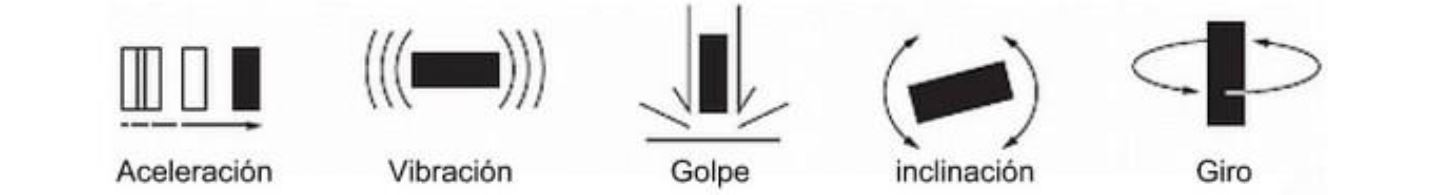
\includegraphics[width=0.8\textwidth]{./img/movimientoAcelera}
	\caption{Movimientos básicos asociados con la aceleración de un objeto. \cite{juanDiego}} 
	\label{fig:movimientosAcelera}
\end{figure} 


A continuación se explica brevemente cada uno de los tres tipos de sensores que incluye una unidad inercial. \cite{juanDiego}

%\newpage %Salto de pagina
	\begin{itemize}
		%-Acelerómetro
		\item \textit{\textbf{Acelerómetro}}	
		% \hspace{0.2cm} 
		\begin{figure}[H]
			\centering
			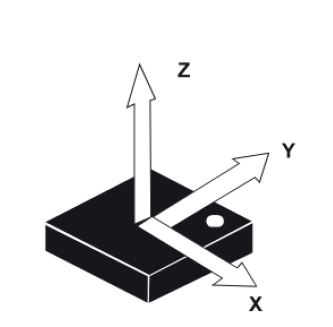
\includegraphics[width=0.25\textwidth]{./img/IMUacelerometro}
			\caption{Lectura de aceleración lineal en los ejes del acelerómetro. \cite{juanDiego}} 
			\label{fig:IMUacelerometro}
		\end{figure} 
		
		El acelerómetro mide la aceleración del objeto al que va unido respecto de una masa inercial interna. Más en concreto, mide la segunda derivada de la posición, la fuerza de inercia que se genera cuando a una masa le afecta un cambio de velocidad.
		
		A la hora de utilizar estos sensores hay que tener en cuenta el valor de la temperatura y frecuencia de funcionamiento, además de la desviación estándar que tenga el sensor específico.
		
		El modelo matemático de un acelerómetro es el siguiente:
		\begin{equation}
			\label{eq:modeloAcelera}
			a = G_{a}\; a_{0} + b_{a} + n_{a}
		\end{equation}
		dónde, $ G_{a} $ y $ b_{a} $ son el factor de escala y el bias o error sistemático proporcionado por el fabricante, $ a_{0} $ es el valor de aceleración medido por el sensor inercial y $ n_{a} $ que es ruido blanco gaussiano.
		
	
		%-Giroscopio
		\item \textit{\textbf{Giroscopio}}	
		% \hspace{0.2cm} 
		
		\begin{figure}[H]
			\centering
			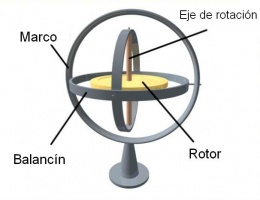
\includegraphics[width=0.35\textwidth]{./img/IMUgiroscopo}
			\caption{Esquema típico de un giroscopio. \cite{juanDiego}} 
			\label{fig:IMUgiroscopo}
		\end{figure} 
		
		Este tipo de sensor sirve para medir la orientación. El principio de funcionamiento de un giroscopio reside en la conservación del momento angular. 
		
		En la fígura \ref{fig:IMUgiroscopo} se observan los cuatro elementos que componen un giroscopio típico. Mientras que en el caso de los acelerómetros se mide la aceleración lineal, en los giróscopos se mide la aceleración angular. El dispositivo con forma esférica tiene en su centro un disco que puede rotar libremente en cualquier dirección sobre su eje de simetría. 
				
		
		
		El modelo matemático de un giroscopio es el siguiente:
		\begin{equation}
			\label{eq:modelogiroscopo}
			\omega = G_{g}\; \omega_{0} + b_{g} + n_{g}
		\end{equation}
		dónde, $ G_{g} $ y $ b_{g} $ son el factor de escala y el bias o error sistemático proporcionado por el fabricante, $\omega_{0} $ es el valor de aceleración angular medido por el sensor inercial y $ n_{g} $ que es ruido blanco gaussiano.
		
			
		%-Magnetómetro
		\item \textit{\textbf{Magnetómetro}}	
		% \hspace{0.2cm} 
		\begin{figure}[H]
			\centering
			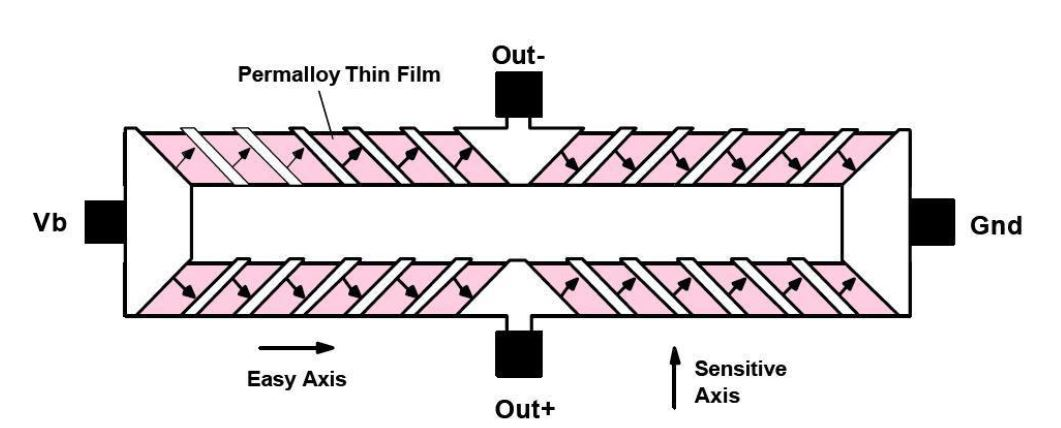
\includegraphics[width=0.55\textwidth]{./img/IMUmagnetometro}
			\caption{Esquema típico de un magnetómetro. \cite{juanDiego}} 
			\label{fig:IMUmagneto}
		\end{figure} 
		
		Mide la intensidad de un campo magnético en tres ejes. De ello se obtiene un vector de campo que da información del ángulo de azimut o de su altitud. Podría decirse que es la función de una brujula en tres dimensiones, con la capacidad de distinguir giros en el eje de roll y pitch. Entender cómo funciona el campo magnético terrestre facilita la comprensión del funcionamiento de este tipo de sensores (\ref{fig:campoMag}).
		
		\begin{figure}[H]
			\centering
			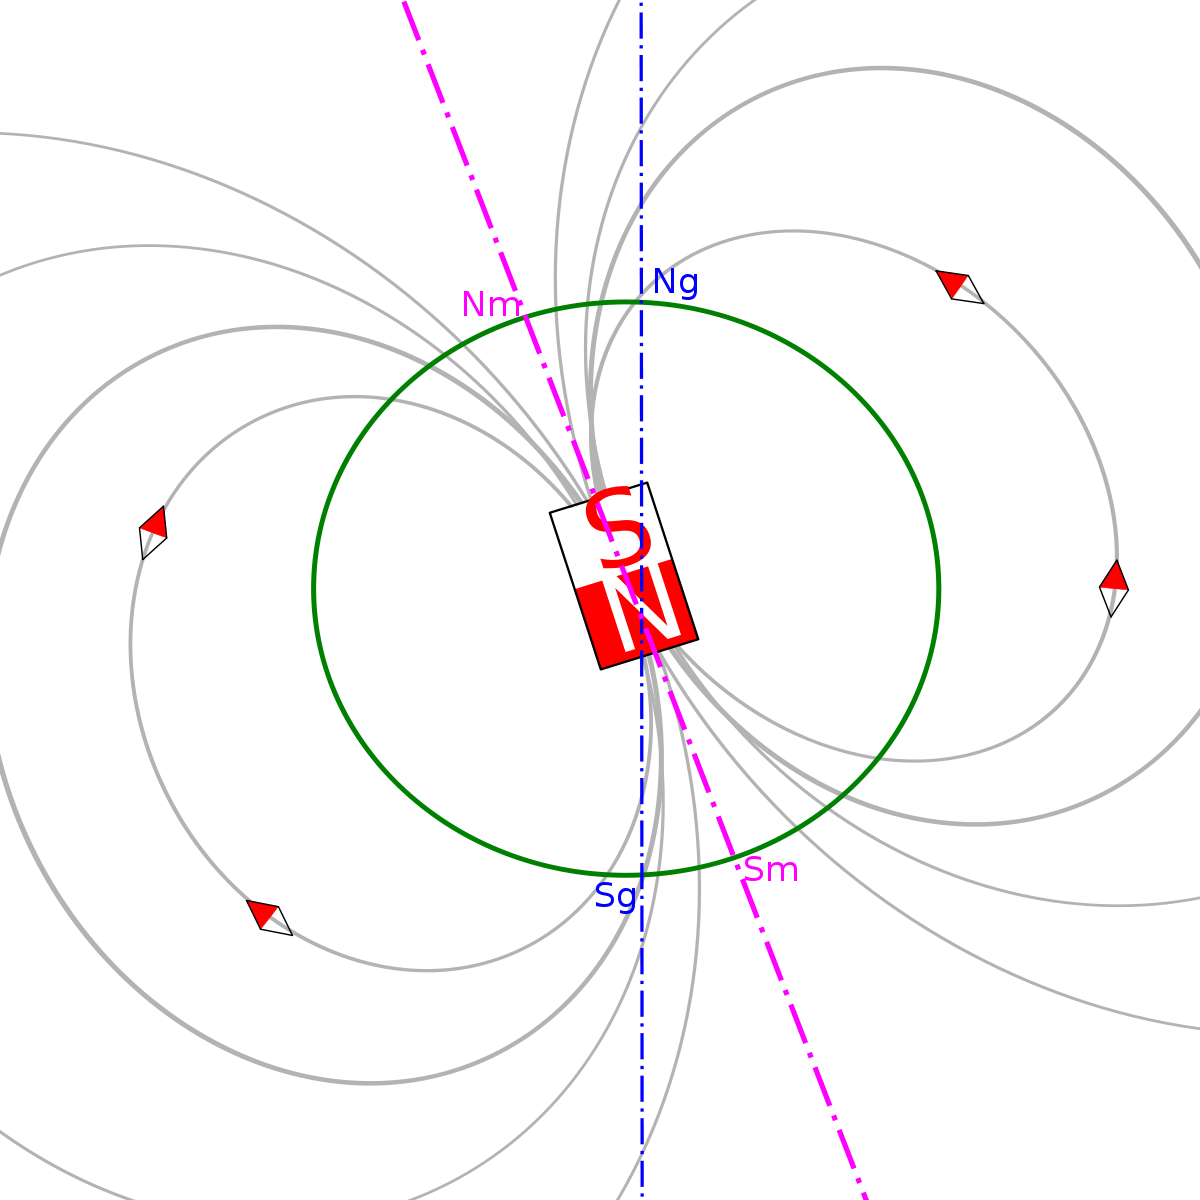
\includegraphics[width=0.55\textwidth]{./img/IMUmagneto}
			\caption{Líneas de campo magnético terrestre referencia Norte-Sur. \cite{juanDiego}} 
			\label{fig:campoMag}
		\end{figure} 
		
		El modelo matemático de un magnetómetro (ecuación \ref{eq:modeloMagneto}) es similar al del acelerómetro y el giroscopio con la diferencia de lo que se mide es intensidad de campo magnético en vez de aceleración. 
		\begin{equation}
			\label{eq:modeloMagneto}
			m = G_{m}\; m_{0} + b_{m} + n_{m}
		\end{equation}
		dónde, $ G_{m} $ y $ b_{m} $ son el factor de escala y el bias o error sistemático proporcionado por el fabricante, $m_{0} $ es el valor de intensidad de campo magnético medido por el sensor inercial y $ n_{m} $ que es ruido blanco gaussiano.
		
		
		
	\end{itemize}
	


\subsection{Microcontrolador basado en ESP32}
\label{sec:esp324}

	\begin{figure}[H]
		\centering
		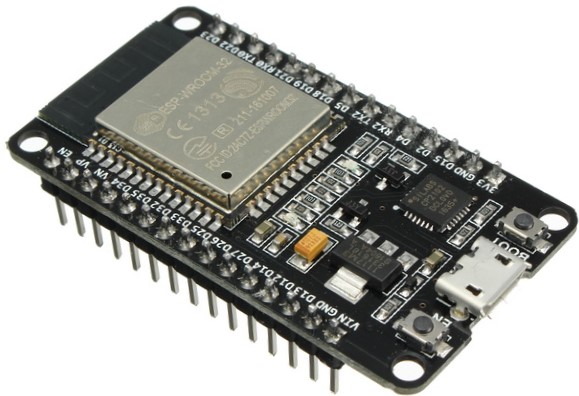
\includegraphics[width=0.4\textwidth]{./img/esp32}
		\caption{Módulo ESP32. } 
		\label{fig:esp32}
	\end{figure} 


\begin{table}[H]
	\centering
	\begin{tabular}{|l|c|}
		\hline
		{\cellcolor[HTML]{EFEFEF}Cores}                                      & 2                             	\\ \hline
		{\cellcolor[HTML]{EFEFEF}Arquitectura}                               & 32 bit                         	\\ \hline
		{\cellcolor[HTML]{EFEFEF}Frecuencia de reloj} 						 & 160 MHz 							\\ \hline
		{\cellcolor[HTML]{EFEFEF}Wifi}                                       & Sí                             \\ \hline
		{\cellcolor[HTML]{EFEFEF}Bluetooth}                                  & Sí                             \\ \hline
		{\cellcolor[HTML]{EFEFEF}RAM}                                        & 512 KB                         \\ \hline
		{\cellcolor[HTML]{EFEFEF}FLASH}                                      & 16 MB                          \\ \hline
		{\cellcolor[HTML]{EFEFEF}Pines GPIO}                                 & 36                             \\ \hline
		{\cellcolor[HTML]{EFEFEF}Buses}                                      & SPI, I2C, UART, I2S, CAN       \\ \hline
		{\cellcolor[HTML]{EFEFEF}Pines ADC}                                  & 18                             \\ \hline
		
	\end{tabular}
	\caption{Tabla de propiedades características ESP32}
	\label{tabla:ESP32}
\end{table}

Se ha elegido el módulo ESP32 (figura \ref{fig:esp32}) frente a otros módulos existentes por sus competentes prestaciones. En la tabla \ref{tabla:ESP32} se resumen sus características más notables. De entre ellas, las que más hacen destacar al ESP32 son la frecuencia de la CPU, el número de cores y la capacidad de conectividad de la que dispone sin necesidad de agregarle dispositivos extra (ver figura \ref{fig:esp32tabla}).


	\begin{figure}[H]
		\centering
		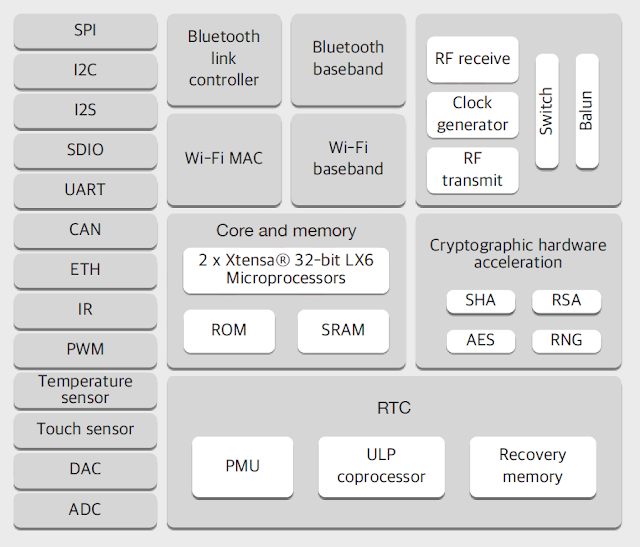
\includegraphics[width=0.8\textwidth]{./img/esp32diagrama}
		\caption{Diagrama de bloques de ESP32. } 
		\label{fig:esp32tabla}
	\end{figure} 

Todo esto sin recurrir a un aumento del tamaño frente a otros módulos de este tipo. El módulo ESP32 mide en torno a los $12\;cm^{2}$ ($ 51 \times 23 mm $) de área.


%--Desarrollo del prototipo
\section{Prototipo propuesto}
\label{sec:prototipo4}

En esta sección se presenta el concepto del prototipo basado en IMUs propuesto.

\subsection{Disposición}
\label{sec:materiales4}

Los elementos fundamentales en esta propuesta son los sensores IMU y el módulo ES32. Se pretende conocer el movimiento de cada una de las falanges de los dedos, el dorso y la muñeca. Para ello se propone colocar los elementos como se muestra en la figura \ref{fig:disposicionIMU}. 


\begin{figure}[H]
	\centering
	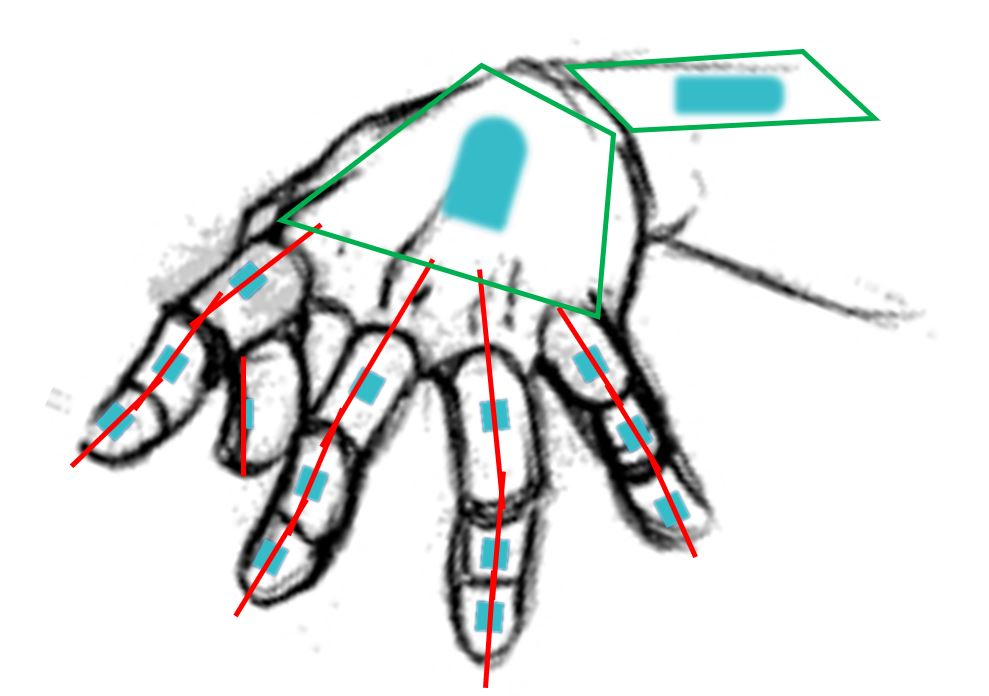
\includegraphics[width=0.6\textwidth]{./img/IMU2}
	\caption{Disposición de los elementos del prototipo sobe la mano. } 
	\label{fig:disposicionIMU}
\end{figure} 

 Lo importante en esta propuesta es que los sensores estén colocados en la falange que le corresponda. Una ventaja de emplear esta distribución junto con esta tecnología es que la colocación exacta de los sensores no influye demasiado al resultado medido. Es decir, si el sensor se encuentra colocado a una distancia diferente de la articulación entre una sesión y otra no alterará el resultado de la medición.

Además, gracias al reducido tamaño del módulo ESP32, este se puede colocar sobre el dorso de la mano o en la muñeca. 

A la hora de elegir los sensores, la característica limitante ha sido el número de direcciones de sus puertos I2C. Por simplificar el cableado, se utilizan los puertos I2C, que permiten conectar en paralelo varios dispositivos al mismo puerto. Para ello cada dispositivo tiene que tener asignada una dirección de lectura. 

Buscando los sensores IMU de nueve grados de libertad (9DOF) se encuentra que sólo se pueden configurar en dos direcciones, la dirección 68 y la 69. Por lo tanto se ha decidido emplear también los IMUs de seis grados de libertad. Este tipo de IMUs (6DOF) no cuentan con la información que da el magnetómetro, teniendo únicamente giroscopio y acelerómetro. Dentro de este tipo de IMUs pasa lo mismo que con los 9DOF, únicamente se encuentran dos direcciones: la 1C-6A y la 1E-6B (dir.acelerómtetro-dir.giroscopio). Hasta este punto se tienen cuatro direcciones diferentes, pero se necesitan más sensores, uno por cada falange más dos por la muñeca y el dorso de la mano.

La solución adoptada ante la falta de disposición de direcciones en los sensores ha sido la utilización de un multiplexor de puertos I2C 1:8. De esta forma se pueden tener 16 IMUs del tipo 6DOF y 16 IMUs del tipo 9DOF. En la figura \ref{fig:esquemaimu} se puede ver como es la conexión de los sensores con el multiplexor y el módulo ESP32. Para simplificar el esquema se ha tomado solamente una de las salidas del multiplexor, el resto se conecta de la misma manera.

\begin{figure}[H]
	\centering
	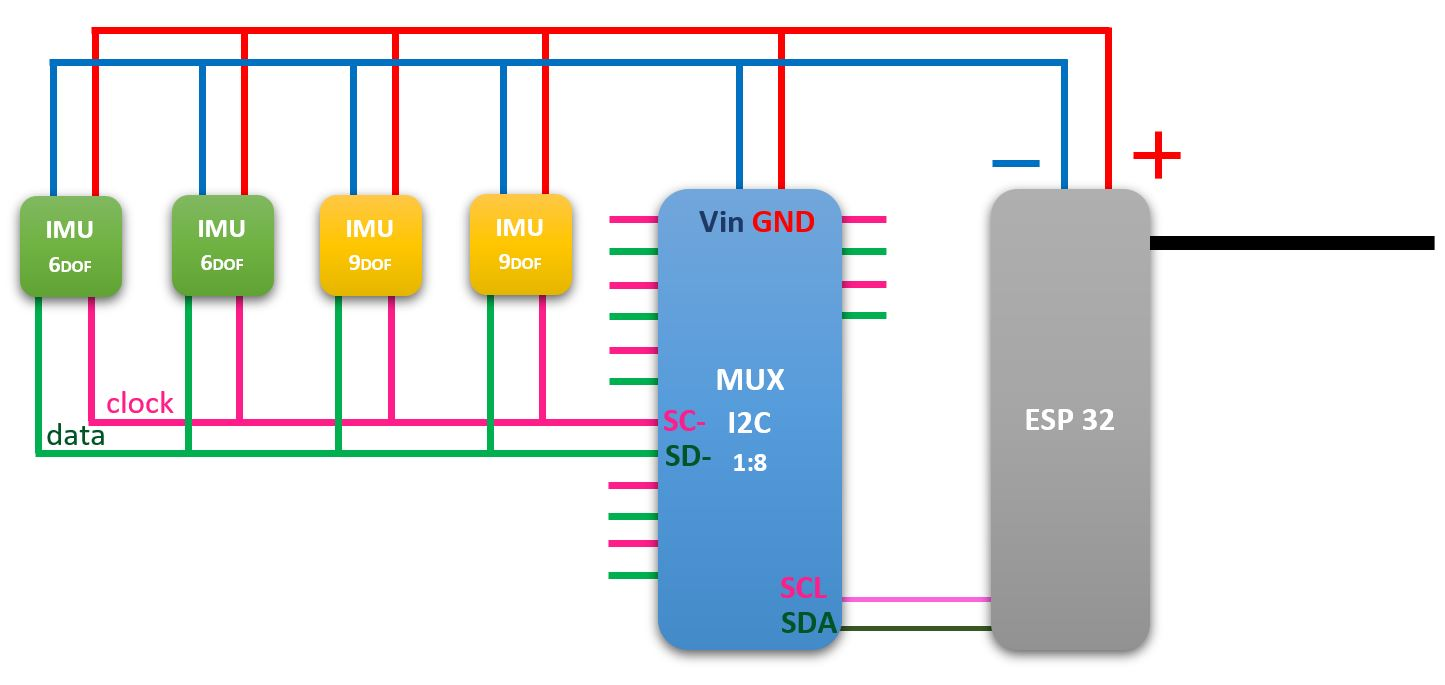
\includegraphics[width=0.95\textwidth]{./img/esquemaimu}
	\caption{Conexión I2C de una de las salidas del multiplexor. } 
	\label{fig:esquemaimu}
\end{figure} 


En el prototipo propuesto se ha decidido utilizar los IMUs 9DOF en la muñeca, el dorso de la mano, la falange distal y medial del pulgar y las falanges proximales del dedo índice, corazón, anular y meñique. Contando con que todos estos puntos utilizan el sistema de referencia global, los sensores 6DOF se reservan para los puntos en los que la referencia global que aporta el magnetómetro es prescindible por la fisionomía de la mano. Siendo estos puntos las falanges distales y mediales de los dedos índice, corazón, anular y meñique. Ver figura \ref{fig:anatomiaMano}


\subsection{Funcionamiento}
\label{sec:funcionamiento4}

Este prototipo funcionará con un software que podrá ser utilizado tanto desde la tableta como el ordenador. 

El módulo ESP32 es el encargado de procesar los datos obtenidos por los sensores y estos datos serían transmitidos (vía cable o wireless) al software en la tableta o PC. Con estos datos será posible hacer una representación en 3D de la disposición de la mano. 

Hay tres pantallas clave que darán una experiencia de uso óptima al fisioterapeuta y el paciente:


\begin{itemize}
	\item \textbf{Pantalla de medición}
	
	\begin{figure}[H]
		\centering
		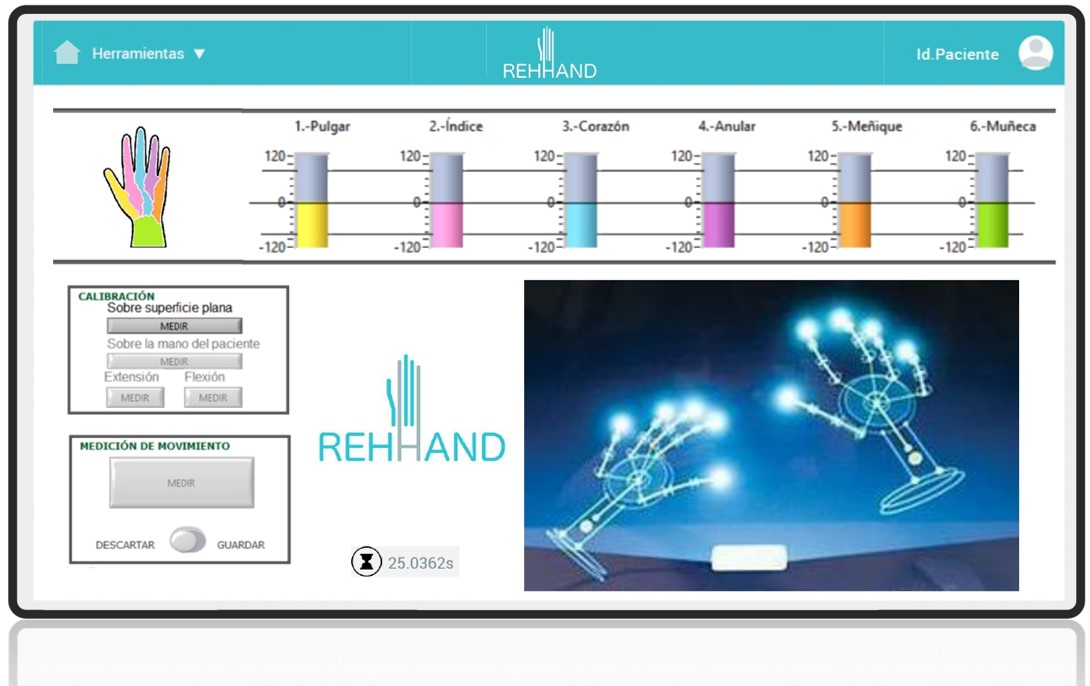
\includegraphics[width=0.65\textwidth]{./img/softwareIMU1}
		\caption{Pantalla de medición de la rehabilitación. } 
		\label{fig:softIMU1}
	\end{figure} 
	 
	 Esta parte del software sirve para las mediciones en los ejercicios de rehabilitación. En el caso de los IMUs es necesaria realizar una calibración antes de comenzar la medición (equivalente a la de "\textit{sobre superficie plana}"), a diferencia del prototipo con FBG.
	 
	 La visualización en pantalla del movimiento mejorará la experiencia de usuario. El sistema permite la visualización de los datos en tiempo real.
	
	\item \textit{Pantalla de análisis de datos}
	
	\begin{figure}[H]
		\centering
		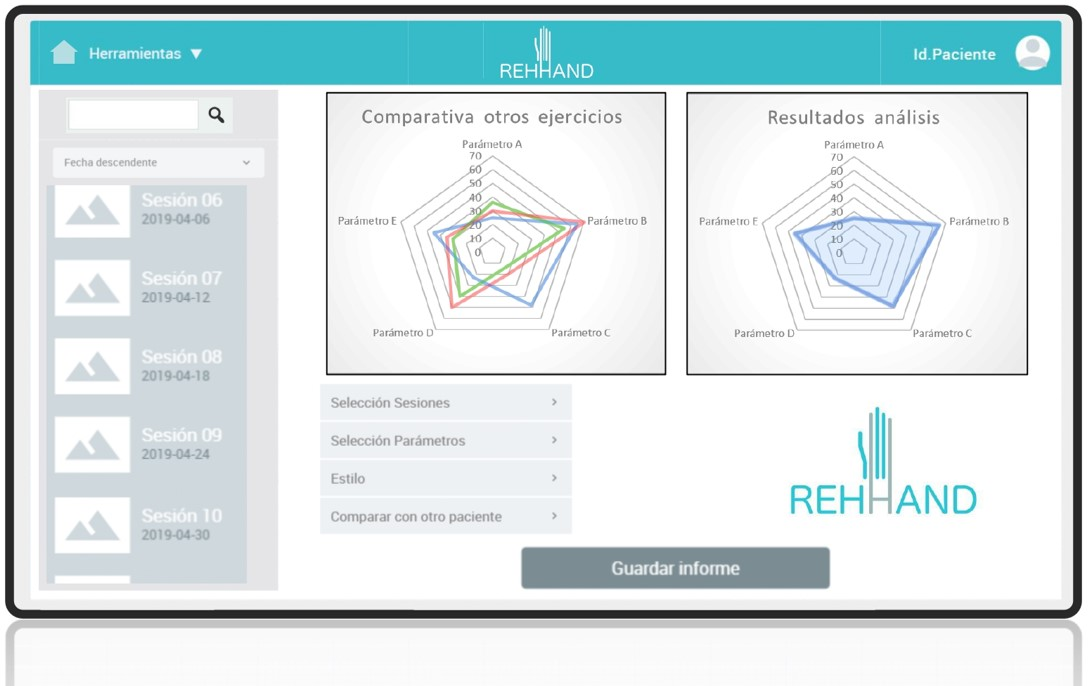
\includegraphics[width=0.65\textwidth]{./img/softwareIMU2}
		\caption{Pantalla de análisis de resultados de las sesiones. } 
		\label{fig:softIMU2}
	\end{figure} 
	
	Esta parte del software permite visualizar los resultados de las sesiones realizadas y comparar los resultados entre ellas. Esto permite tener un conocimiento real del avance de la rehabilitación y fijar nuevos objetivos en el proceso de recuperación del paciente. Gracias a esta forma de visualizar los datos el paciente será consciente de su evolución influyendo en su motivación a la hora de realizar los ejercicios de rehabilitación.
 
	
	
	\item \textbf{Pantalla de minijuegos}
	
	\begin{figure}[H]
		\centering
		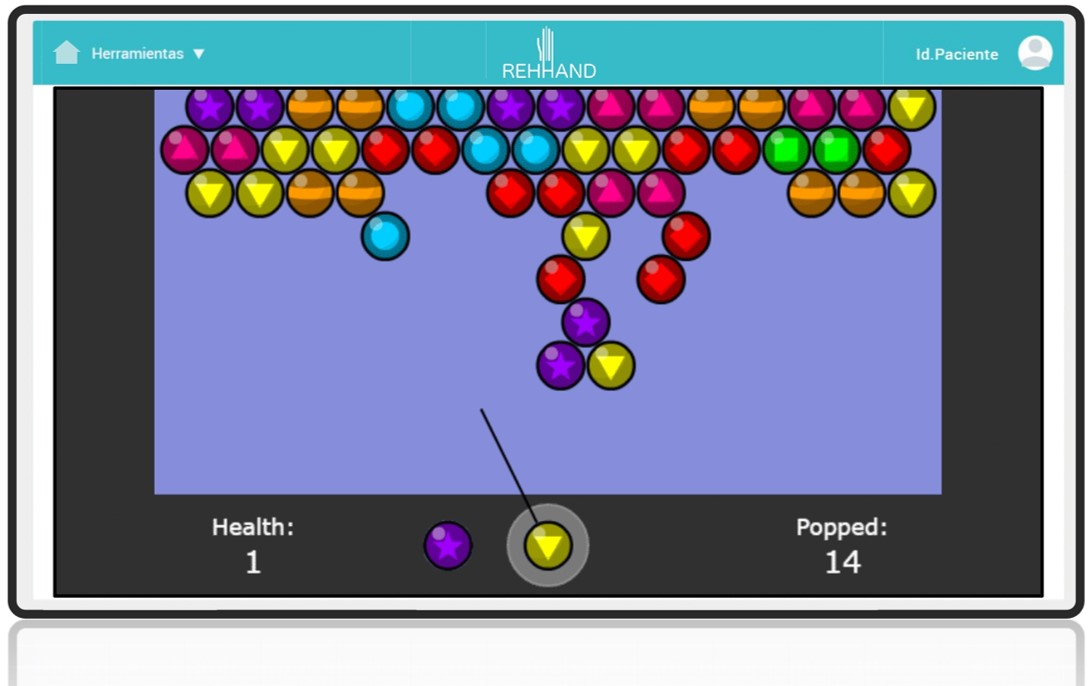
\includegraphics[width=0.65\textwidth]{./img/softwareIMU3}
		\caption{Pantalla de medición de la rehabilitación. } 
		\label{fig:softIMU3}
	\end{figure} 
	
	Esta última ventana consistirá en una colección ampliable de minijuegos controlados por el movimiento de los sensores de la mano. Puesto que no todos los pacientes tienen el mismo rango de movimiento, en una ventana previa se ajustará el rango del juego al rango articular del usuario.
	
	Esta funcionalidad del software, es la que sirve como entrenamiento para los pacientes. 
	
	
\end{itemize}




\section{Resultados y análisis}
\label{sec:resultados4}

   
	
	Esta solución tiene como principal ventaja frente a la basada en FBGs que las mediciones con los IMUs permiten llevar un seguimiento del paciente entre sesiones al utilizar un sistema de referencia global. Además, el software es más versatil, permitiendo diseñar funcionalidades más complejas y una entorno de trabajo más vistoso.
 
	
	Conviene realizar una comparativa económica para entender la diferencia de precio entre ambas propuestas. En la figura \ref{fig:precioCompara} se presentan los precios aproximados de los componentes fundamentales de cada prototipo. En ninguno se ha tenido en cuenta el precio de la estructura del guante ni el cableado. Es importante mencionar la gran diferencia de coste entre un prototipo y otro.
	
	\begin{figure}[H]
		\centering
		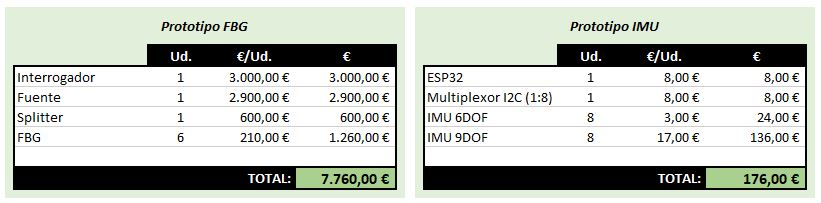
\includegraphics[width=\textwidth]{./img/precios2}
		\caption{Precios orientativos de los componentes en el prototipo basado en FBG y en el basado en IMUs. } 
		\label{fig:precioCompara}
	\end{figure} 
	
	
	